\section{Quadratic Relations}

Among all convex bifunctions, quadratic ones are particularly well-structured:
they are the simplest class rich enough to express least-squares problems, energy minimisation, and Gaussian inference, yet structured enough to admit a finite diagrammatic presentation. This section develops the Graphical Quadratic Algebra (GQA) \cite{stein2024gqa}, the first of the two graphical theories on which our linear programming algebra will be built.
We begin with the necessary preliminaries on quadratic functions, then define the symmetric monoidal theory whose morphisms are non-negative quadratic optimization problems — the non-negativity condition ensuring that infimal composition is always well-posed. We then present the soundness and completeness results for this theory. The section closes by deriving several known results about quadratic problems purely through string diagram manipulation, demonstrating that the graphical syntax is not merely a notational convenience but a genuine calculus in which optimization arguments can be carried out.
\subsection{Preliminary results about quadratic functions}

Our main interest are non-negative quadratic functions. The motivation for this
unusual choice is that we want to avoid unbounded problems remain on convex settings, since negative quadratic functions
may be concave. Formally,
this means that the category of partial non-negative quadratic functions embeds into the positive
Lawvere-quantale.

Next, we rigorously define the notion of a non-negative quadratic function
along with other relevant equivalence results.

\begin{definition}
    A partial quadratic function is a function
\[
f : \mathbb{R}^{n+m} \to [0,+\infty]
\]
of the form
\[
f(x,y) = \langle x, Ax\rangle + \langle b, x\rangle + c +\{| x \in M|\}
\]
where $A$ is a symmetric matrix, $M$ is an affine subspace, $b \in \mathbb{R}^n$ and $c \in \mathbb{R}$ and $\langle-,-\rangle$ denotes the usual inner product on the reals.
\end{definition}

\begin{definition}
    An elementary convex partial quadratic function $h$ is a function that can be written in the diagonal form $h(x) = \sum_i \lambda_i x_i^2$ for $\lambda_i \ge 0$. It is partial because $h(x) = \infty$ whener $\lambda_i = +\infty$ $x_i \neq 0$ for some $i$.
\end{definition}

\begin{proposition}\label{prop:PQFEquivalence}
    The following statements are equivalent
    \begin{itemize}
        \item $f$ is a non-negative partial quadratic function
        \item $f$ can be written in the form $f(x) = h(A(x-a)) + c$ where $A$ is an invertible matrix, $c \ge 0$ and $h$ an elementary convex partial quadratic function
        \item $f$ can be written as $f(x) = \inf \{ ||y||^2: (x,y) \in M\}$ where $M$ is an affine subspace
    \end{itemize}
\end{proposition}


\begin{proof}[Proof of Proposition 2]

\noindent
\textbf{(1) $\Rightarrow$ (2).}
Using an affine change of coordinates, we may assume that the domain of $f$
is the subspace
\[
M=\mathbb{R}^m \times \{0\}.
\]
Define the restricted function
\[
\tilde f(x_1,\dots,x_m)
=
f(x_1,\dots,x_m,0,\dots,0).
\]
Then $\tilde f$ is a total nonnegative quadratic function. Hence, by the
characterisation of total nonnegative quadratic functions,
there exist an invertible matrix $A$, a vector $a$, a constant $c\ge 0$,
and an elementary convex quadratic function $h$ such that
\[
\tilde f(x_1,\dots,x_m)
=
h\big(A((x_1,\dots,x_m)-a)\big)+c.
\]
Returning to the original coordinates, we obtain
\[
f(x)
=
h\big(A((x_1,\dots,x_m)-a)\big)
+ \infty \cdot x_{m+1}
+ \cdots
+ \infty \cdot x_n
+ c,
\]
which is of the required form.

\medskip
\noindent
\textbf{(2) $\Rightarrow$ (3).}
Under the affine coordinate change
\[
y = A(x-a),
\]
it suffices to consider functions of the form
\[
f(y)=h(y)+c,
\]
where $h$ is an elementary quadratic function. Up to a permutation of
coordinates, we may write
\[
h(y_1,y_2,y_3)
=
\|y_1\|_2^2
+
\{\, y_3=0 \,\},
\]
where $\{\, y_3=0 \,\}$ denotes the indicator function of the subspace
$\{y_3=0\}$ (equal to $0$ if $y_3=0$ and $+\infty$ otherwise).

Define the affine relation
\[
M
=
\left\{
\big((y_1,y_2,y_3),(y_1,\sqrt{c})\big)
\;\middle|\;
y_3=0
\right\}.
\]
Then, for every $x$,
\[
f(x)
=
\inf\{\|z\|_2 : (x,z)\in M\}.
\]

\medskip
\noindent
\textbf{(3) $\Rightarrow$ (1).}
Let $M\subset \mathbb{R}^n\times\mathbb{R}^m$ be an affine relation.
Then there exists a vector subspace $D\subset \mathbb{R}^m$ and an affine map
$g:\mathbb{R}^n\to D^\perp$ such that, for each $x$,
\[
M_x
=
\{y : (x,y)\in M\}
=
\begin{cases}
g(x)+D, & x\in \pi_X M,\\
\varnothing, & \text{otherwise},
\end{cases}
\]
where $\pi_X M$ denotes the projection of $M$ onto $\mathbb{R}^n$.

Hence,
\[
\inf\{\|y\|_2 : y\in M_x\}
=
\|g(x)\|_2
+
\{\, x\in \pi_X M \,\}.
\]
This is clearly a nonnegative partial quadratic function.
\end{proof}

As it is stated above, a non-negative partial quadratic function has a very convenient algebraic
structure that can be expressed both with and without explicit constrains.

This formulation reveals one of the deepest conceptual payoffs of the relational framework.  In the standard convex analysis view \cite{boyd2004convex}, incorporating a constraint
$y \in M_x$ into an objective function via its indicator
\[
\inf\{\|y\|_2 : y\in M_x\}
=
\inf_y \big\{\|y\|_2 + \mathbf{1}_{M}(y) \big\}
\]
is a familiar technique, closely related to the method of Lagrangian multipliers.  In the relational setting, however, this operation acquires a precise categorical meaning:
binary relations, identified with their $\{0,+\infty\}$-valued characteristic functions,  represent the \emph{feasibility constraints} of an optimization problem, while weighted
relations represent its \emph{objective function}. Composing the two --- adding the  indicator to the cost --- is precisely categorical composition in $\mathbf{BiFunc}$.
Constraints and objectives are therefore not fundamentally different kinds of objects:  they are relations valued in different quantales, unified by the same compositional
structure.

This correspondence is made precise by the following proposition, which  establishes that non-negative partial quadratic functions are closed under  the categorical composition of $\mathbf{CxBiFn}$.

\begin{proposition}\label{prop:partial quadratic composition}
    If $M \subseteq \mathbb{R^n} \times \mathbb{R^m}$ is an affine subspace, and $g$ is a non-negative partial quadratic function, then so is $f(x) = \inf \{g(y)\; |\;(x,y)\in M\} $
\end{proposition}

\begin{proof}
Let $g:\mathbb{R}^m \to [-\infty,\infty]$ be a nonnegative partial quadratic
function and let $M \subseteq \mathbb{R}^m \times \mathbb{R}^n$ be an affine
relation. Using the representation of Proposition~16 and an affine change of
coordinates, it suffices to consider the case where $g$ is an elementary
function. Hence we may assume that $g$ is given by a constrained minimization
problem of the form
\[
f(x)
=
\inf \left\{
\|y_1\|_2^2 + \{\, y_3 = 0 \,\}
\;\middle|\;
(x,(y_1,y_2,y_3)) \in M
\right\}.
\]

Define the affine relation
\[
M'
=
\left\{
(x,y_1)
\;\middle|\;
(x,(y_1,y_2,0)) \in M
\right\}.
\]
Since $M$ is affine, it follows directly that $M'$ is also an affine
relation. Moreover, the constraint $\{\, y_3 = 0 \,\}$ has been incorporated
into the definition of $M'$.

Therefore,
\[
f(x)
=
\inf
\left\{
\|y\|_2^2
\;\middle|\;
(x,y) \in M'
\right\},
\]
which is of the form characterizing partial quadratic functions. Hence
$f$ is a partial quadratic function.

\end{proof}
The above result is the closure property that makes graphical theory well-founded: the composition of a quadratic objective with any number of  affine constraints remains a quadratic problem. In other words, we can compose a weighted relation with as many affine relations as we want. This is equivalent of adding affine constrains to the problem.

Categorically, it states  that non-negative partial quadratic functions form a subcategory of  $\mathbf{CxBiFn}$ that is closed under infimal composition, and it is  precisely this subcategory that the Graphical Quadratic Algebra axiomatises.

%%%%%%%%%%%%%%%%%%%%%%%%%%% GQA ALGEBRA %%%%%%%%%%%%%%%%%%%%%%%%%%%%%%
\subsection{Graphical Algebra for quadratic problems}\label{sec:gqa}

We now introduce the first axiomatic algebra of the thesis: the Graphical  Quadratic Algebra (GQA) \cite{stein2024gqa}. The goal of this diagrammatic  calculus is to express and reason about optimization problems with non-negative  quadratic objective functions and equality constraints. The canonical example  of this class is the ordinary least-squares (OLS) estimator
\[
\min_x \| Ax - b \|^2,
\]
whose solution is given by the Moore--Penrose pseudoinverse $A^\dagger$.  This is a problem of central importance in linear algebra, statistics, and  control, and it serves as the principal worked example for GQA: later in  this section we provide a purely diagrammatic argument showing that  $A^\dagger$ solves the least-squares problem.

We proceed as follows. We first define the symmetric monoidal theory  $(\Sigma_{\mathrm{GQA}}, E_{\mathrm{GQA}})$ by specifying its generators  and equations. We then define the semantic category $\mathbf{QuadRel}$ of  non-negative quadratic relations, and prove that $\mathbf{GQA}$ axiomatises  it — that is, that the induced PROP morphism is full, faithful, and  essentially surjective. The syntax is built on the following generators  and equations $E$.

\begin{definition}[Graphical Quadratic Theory]

We call $\textbf{GQA}$ the symmetric monoidal theory $(\Sigma,E)$, such that,  $\Sigma$ is depicted graphically as:

\begin{figure}[H]
    \centering
    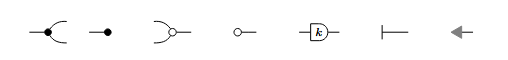
\includegraphics[width=1\linewidth]{images/GQA/GQA.png}
\end{figure}

\medskip

$\Sigma$-terms are defined by vertical and horizontal composition of terms with matching arity and coarity, and are modularized by $E$:

\begin{figure}[H]
    \centering
    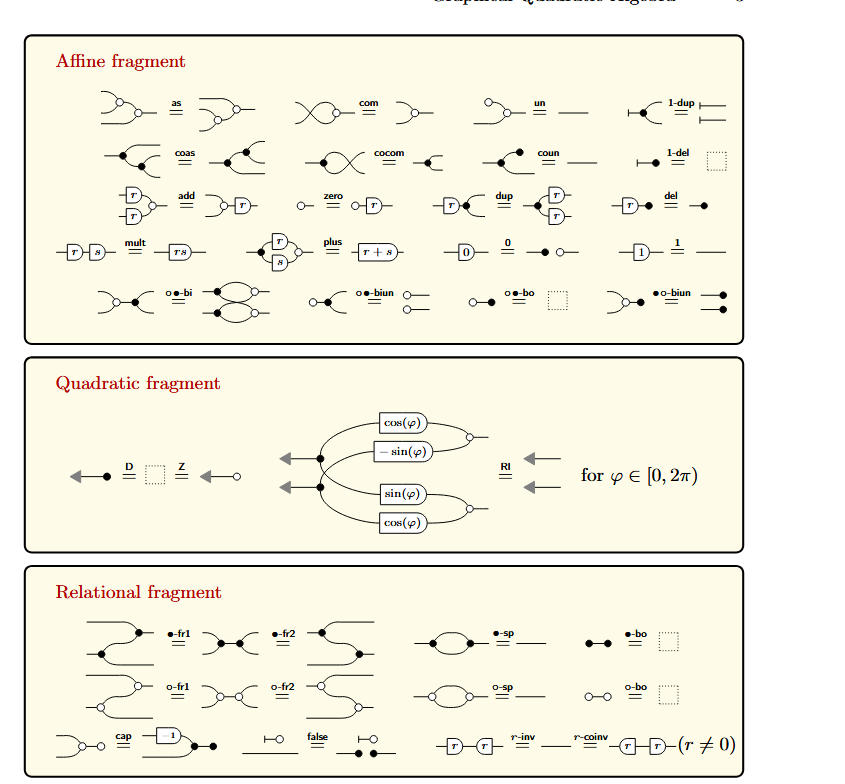
\includegraphics[width=1\linewidth]{images/GQA/GQAAxioms.png}
\end{figure}

The pair $(\Sigma,E)$ defines the symmetric monoidal theory generated by
the operators $\Sigma$ subject to the equations $E$.

We will define the interpretation functor $[ -]$, i.e., the semantics of each generator, as follows:

\begin{figure}[H]
    \centering
    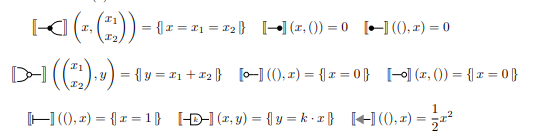
\includegraphics[width=1\linewidth]{images//GQA/GQAInterpretation.png}
\end{figure}

The interpretation of any $\Sigma$-term is, therefore, the vertical(tensor product) and horizontal(categorical composition) combination of the interpretation of each generator that composes it.
\end{definition}

Thus, \textbf{GQA} is an extension of the previous algebra for affine relations \textbf{GAA}.
The extension is done through the addition of a new generator, the gray arrow generator, and its associated axioms.
This is of particular interest, because is the interpretation of such generator
that is lifting the category to the level of weighted relations instead of binary relations.

To understand its role, recall that every generator of $\mathbf{GAA}$ is  interpreted
as the indicator function of some affine subspace. In this  picture, one may think of
numbers flowing along the wires, and each diagram  as encoding membership in some affine set.
The gray arrow  generator behaves differently, rather than enforcing a constraint on the
values running through the wire, it \emph{measures} them and produces a  real-valued output.
No number is transformed inside it; instead, a cost is  emitted.

A useful analogy comes from Electronics.
An electric circuit diagram is a formal diagram that allows you to represent an electric
circuit with wires and devices attached to those wires. In general,
what you see is current running in the wires and some components along it that alter the current. However,
one may attach a measurement device, like an ammeter, in the circuit.
That does not change the current, but it measures it, and outputs a number to outside the diagram.

Distinctively, the syntax admits an alternative probabilistic interpretation.
Under this reading, the gray arrow generator encodes the information of a Gaussian distribution
with mean 0,
its semmantics being that of the function $(\bullet, x)  \mapsto \mathcal{N}(0,x)$; categorically
this encodes the notion of a state in Markov Categories \cite{stein2023gaussian,Cho_2019, fritz2020synthetic}. Hence, \textbf{GQA}
expresses linear functions of random variables, more precisely of normally distributed random variables,
algebraically, turning composition into the act of probabilistic conditioning.

This interpretation of the syntax alludes to the understanding of the new added
generator as the act of observing a particular random variable, thus getting a number out of it.
Although such an extension is not explored in this work, we encourage the interested reader to pursue this
direction \cite{stein2024gqa,stein2025compositional}. We believe there exists a very strong interconnection between
the algebraic semmantics of optimization and that of probabilistic programming \cite{stein2024compositional}, the notion
of measuring in the convex setting being equivalent to that of observing the value of a random variable
in the stochastic one, and the composition playing the role of variable elimination in the first and
of conditioning in the latter. This lacks formality however, and we leave it to future works.

This provides a very meaningful intuition on how to interpret the new generator.
Rather then transforming the values carrieds by wires, the grey arrow generator measures
them and emits a real-valued cost. In this case,
the semantics of the diagram is $(x, \bullet) \mapsto \frac{1}{2}\|x\|^2$,
it measures the l2 norm of the number in the wires. This observation is central, since
the idea of a generator that "measures" or to "outputs" values carried by wires
is the conceptional foundation in our theory of Linear Programming develop in Section~\ref{sec:glp}.

Taking all the $\Sigma$-terms and quotient by their axioms $E$ we generate the free PROP of quadratic diagrams.

\begin{definition}[The Free category of quadratic diagrams]
    We call $\text{FreeP}_{\textbf{GQA}}$ the category of string diagrams of $\textbf{GQA}$
\end{definition}

Observe that we have associated to each generator of $\Sigma$ a visual  diagram. This can be made precise through the notion of a  \emph{strict monoidal functor}. Concretely, the Joyal--Street coherence  theorem \cite{joyal1991geometry} provides a canonical isomorphism of  categories
\[
  \mathbf{FreeP}_{\mathbf{GQA}} \;\xrightarrow{\;\sim\;}\; \mathbf{Diag}(\Sigma),
\]
where $\mathbf{Diag}(\Sigma)$ is the category of isotopy classes of  string diagrams generated by $\Sigma$. Under this isomorphism, each  generating morphism $g \in \Sigma$ is sent to the box labelled $g$ with  its input and output wires, composition $\circ$ is sent to vertical  stacking of diagrams, and the tensor product $\otimes$ is sent to  horizontal juxtaposition. The fact that this assignment is a  \emph{functor} is precisely what guarantees that diagrammatic reasoning  is sound: any equation derivable from the axioms of $\mathbf{GQA}$  holds if and only if the corresponding diagrams are related by  isotopy.

With the syntax in place, we now construct the corresponding semantic  category. As established in the preceding section, the objects of interest  are non-negative partial quadratic functions, or equivalently, quadratic  optimization problems with equality constraints whose objective is bounded  below by zero. These are encoded as \emph{quadratic relations} where $x \in \mathbb{R}^n $ is related to $y \in \mathbb{R}^m$ through a partial non-negative quadratic function
\[
f : \mathbb{R}^n \times \mathbb{R}^m \to [0,+\infty],
\]
where $f(x,y)$ is interpreted as the quadratic cost associated to the pair
$(x,y)$, with $f(x,y) = +\infty$ indicating infeasibility. The following definition constructs the categorical equivalent of such notion.

\begin{definition}[$\mathbf{QuadRel}$]

We define $\mathbf{QuadRel}$ as follows.

\medskip

\noindent
\textbf{Objects.}
Objects are natural numbers $n \in \mathbb{N}$, interpreted as the
Euclidean space $\mathbb{R}^n$.

\medskip

\noindent
\textbf{Morphisms.}
A morphism
\[
f : n \to m
\]
is a partial non-negative quadratic function

\medskip

\noindent
\textbf{Composition.}
Given
\[
f : n \to m,
\qquad
g : m \to k,
\]
their composite
\[
g \circ f : n \to k
\]
is defined by partial minimisation:
\[
(g \circ f)(x,z)
=
\inf_{y \in \mathbb{R}^m}
\left(
f(x,y) + g(y,z)
\right).
\]

\medskip

\noindent
\textbf{Identities.}
For each $n$, the identity morphism
\[
\mathrm{id}_n : n \to n
\]
is given by the quadratic form
\[
\mathrm{id}_n(x,y) =
\begin{cases}
0 & \text{if } x=y, \\
+\infty & \text{otherwise}.
\end{cases}
\]

\medskip

\noindent
\textbf{Monoidal structure.}
The tensor product on objects is addition:
\[
n \otimes m := n+m.
\]

For morphisms
\[
f : n_1 \to m_1,
\qquad
g : n_2 \to m_2,
\]
their tensor product
\[
f \otimes g : n_1+n_2 \to m_1+m_2
\]
is defined by
\[
(f \otimes g)(x_1,x_2,y_1,y_2)
=
f(x_1,y_1) + g(x_2,y_2).
\]

\medskip

From Proposition \ref{prop:partial quadratic composition}, composition is well defined. With these operations, $\mathbf{QuadRel}$ forms a symmetric monoidal
category (indeed a PROP).

\end{definition}

To prove that $\mathbf{GQA}$ presents $\mathbf{QuadRel}$, we require  several preliminary results. A central ingredient in completeness proofs  of this kind is the existence of a \emph{normal form}: a canonical  diagrammatic representation to which every morphism in the category can  be reduced by applying the axioms of the algebra.

The structure of the normal form is typically guided by the key  computational primitive of the semantic category in question. For example,  in $\mathbf{GLA}$, every linear relation can be represented by a pair of  matrices $A, B$ such that
\[
(x,y) \in R
\iff
Ax = By
\iff
[A \;-B] \begin{bmatrix} x \\ y \end{bmatrix} = 0
\iff
\widetilde{A}\,\widetilde{x} = 0,
\]
and the reduction to normal form proceeds through a diagrammatic argument  that mirrors Gaussian elimination on the underlying linear system.

In the quadratic setting, the analogous role is played by the
$QR$  factorization.
Just as Gaussian elimination reduces a linear relation to  a
canonical matrix kernel form, $QR$ factorization reduces a
quadratic  diagram to a canonical form by orthogonally decomposing the underlying  matrix.
This is the appropriate primitive because the objective function  $\|y\|^2$
is invariant under orthogonal transformations, so the axioms  of $\mathbf{GQA}$
can simulate $QR$ steps diagrammatically. The following  results make this precise.

\begin{proposition}\label{prop:projection}
    If $S,D$ are complementary subspaces, then we can prove that:
    \begin{figure}[H]
        \centering
        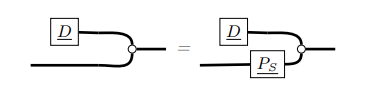
\includegraphics[width=1\linewidth]{images/GQA/subspaceProj.png}
    \end{figure}
\end{proposition}
\begin{proof}
    From the fact that $P_S + P_D = I$, such that $P_S, P_D$ are the projection matrices over
    subspaces $S$ and $D$, we show:

    \begin{figure}[H]
        \centering
        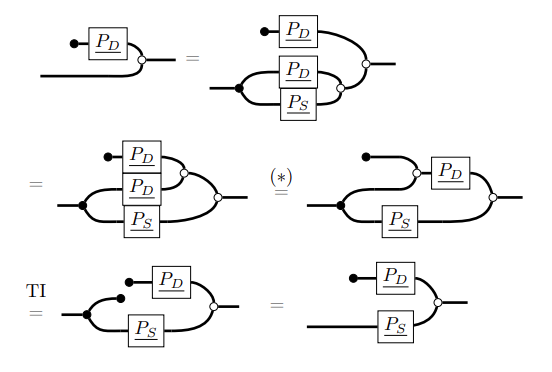
\includegraphics[width=1\linewidth]{images/GQA/ProofProjection.png}
    \end{figure}
\end{proof}

Above result is an analogous way of saying that:
$\{(x,y)|\exists z \in D, z+x =y \} = \{(x,y)|\exists z \in D, z = y - x\}$,
by the orthogonal unique decomposition theorem
$\{(x,y)|\exists z \in D, z = y - x_S - x_D \} = \{(x,y)|\exists z \in D, z + x_D = y - x_S\}$
Since $x_D,z \in D \implies x_D + z = \tilde{z} \in D$ and, by the uniqueness of the decomposition,
$y = \tilde{z} + x_S \implies \tilde{z} = y_D, y_S = x_S$.
$\{(x,y)|\exists \tilde{z} \in D, \tilde{z} = y - x_S\}$.
Visually, one can interpret above diagram as the idea that summing a dangling wire with a
subspace $D$ is equivalent to ask for a pair $(y_{D^\perp}, y)$.

The following remmark establishes a preliminary normal form for the
directed fragment $\overrightarrow{\mathbf{GQA}}$, which will serve as
the key stepping stone toward the full normal form theorem. Intuitively,
it says that any diagram in this fragment can be reorganised into a
canonical block structure determined by a subspace $S$ and compatible
matrix data.

\begin{remark}\label{rmk:normalformgqa}
    Let $M$ be any diagram generated by the fragment
    $\overrightarrow{\mathbf{GQA}}$ (recall Definition~\ref{def:arrows})
    together with the generator $\bullet-$. By collecting terms, we can
    write it as a diagram of the form
    \begin{figure}[H]
        \centering
        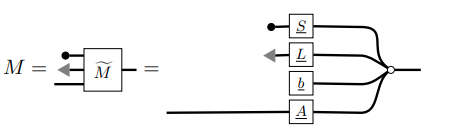
\includegraphics[width=1\linewidth]{images//GQA/GQAeNormalForm.png}
    \end{figure}
    such that $S \subseteq \mathbb{R}^n$ is a vector subspace,
    $b \in S^\perp$, $\operatorname{im}(LL^\top) \subseteq S^\perp$,
    and $\operatorname{im}(A) \subseteq S^\perp$(By Proposition~\ref{prop:projection}).
\end{remark}

\begin{proposition}\label{prop:quadrel_equiv}
Let $N$ be a diagram in the followinf form
    \begin{figure}[H]
        \centering
        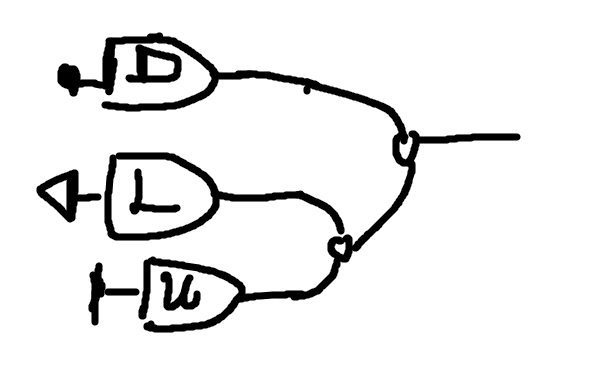
\includegraphics[width=1\linewidth]{images//GQA/preliminary form.png}
    \end{figure}
with data $(D, \mu, L)$, where
$D \subseteq \mathbb{R}^n$ is a vector subspace, $\mu \in D^\perp$,
$L$ is a lower-triangular matrix with
and $\operatorname{im}(LL^\top) \subseteq D^\perp$.
Its semantic interpretation in $\mathbf{QuadRel}$ is the partial
non-negative quadratic function
\[
[N](x)
= \tfrac{1}{2}(x - \mu)^\top L L^\top (x - \mu) + \{|D^\perp + \mu|\}(x),
\]
Moreover, two canonical block-form diagrams $N_1$, $N_2$ with data
$(D_1, \mu_1, L_1)$ and $(D_2, \mu_2, L_2)$ satisfy
$[N_1] = [N_2]$ in $\mathbf{QuadRel}$ if and only if
\[
D_1 = D_2, \qquad \mu_1 = \mu_2, \qquad L_1 L_1^\top = L_2 L_2^\top.
\]
\end{proposition}

\begin{proof}
The first claim follows by direct computation of the interpretation
functor $[-]$ applied to the block form. The $L$-block contributes
the quadratic term $\tfrac{1}{2}(x-\mu)^\top LL^\top(x-\mu)$, the
subspace $D$ contributes the indicator $\iota_{D^\perp}$, and the
vector $\mu$ shifts the centre of the feasible region.

For the equivalence, the $(\Leftarrow)$ direction is immediate from
the first claim. For $(\Rightarrow)$, suppose $[N_1] = [N_2]$
pointwise on $\mathbb{R}^n$.

The domain of finiteness of $[N_i]$ is the affine subspace
$D_i^\perp + \mu_i$. Since $[N_1] = [N_2]$, these domains coincide:
$D_1^\perp + \mu_1 = D_2^\perp + \mu_2$. Two cosets are equal only
if their direction subspaces agree, so $D_1^\perp = D_2^\perp$,
hence $D_1 = D_2$. Write $D := D_1 = D_2$.

The coset equality now gives $\mu_1 - \mu_2 \in D^\perp$.
Evaluating both functions at $x = \mu_1$:
\[
0 = [N_1](\mu_1) = [N_2](\mu_1)
  = \tfrac{1}{2}(\mu_1 - \mu_2)^\top L_2 L_2^\top (\mu_1 - \mu_2).
\]
Since $L_2 L_2^\top$ is positive semidefinite and its restriction to
$D^\perp$ is positive definite (as $\operatorname{im}(L_2 L_2^\top)
\subseteq D^\perp$ with $L_2$ of full rank on $D^\perp$), the
equation above forces $\mu_1 - \mu_2 = 0$, i.e.\ $\mu_1 = \mu_2$.

With $D_1 = D_2$ and $\mu_1 = \mu_2 =: \mu$ established, the identity
$[N_1](x) = [N_2](x)$ for all $x \in D^\perp + \mu$ yields
\[
(x - \mu)^\top L_1 L_1^\top (x - \mu)
= (x - \mu)^\top L_2 L_2^\top (x - \mu)
\qquad \forall\, x \in D^\perp + \mu.
\]
Setting $v = x - \mu \in D^\perp$, this is a quadratic identity on
$D^\perp$. By polarisation it implies $L_1 L_1^\top = L_2 L_2^\top$
as operators on $D^\perp$, and since both sides vanish on $D$, equality
holds on all of $\mathbb{R}^n$.
\end{proof}

We now state and prove the main normal form theorem for $\mathbf{GQA}$.
The theorem states that every
diagram can be decomposed into a purely relational part — a morphism in
$\mathbf{GQA}$ — and a non-negative scalar, corresponding respectively to
the constraint structure and the quadratic cost of the underlying
optimization problem. The proof proceeds by a diagrammatic version of
$QR$ factorization: orthogonal transformations are simulated by axiom
applications, progressively eliminating generators until the canonical
form is reached.

\begin{theorem}[\textbf{GQA} Normal Form]
    Every diagram $M \in \overrightarrow{\mathbf{GQA}}$ can be rewritten,
    modulo the axioms $E$, as $M' \otimes c$ where $M' \in \mathbf{GQA}$
    and $c \in [0,+\infty]$ is a scalar of the form:
    \begin{figure}[H]
        \centering
        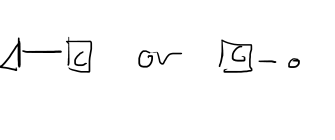
\includegraphics[width=.75\linewidth]{images//GQA/NormalFormScalar.png}
    \end{figure}
\end{theorem}

\begin{proof}
    In a hypergraph category, there is a bijection between
    $\mathrm{Hom}(c,d)$ and $\mathrm{Hom}(\mathbb{1}, c \otimes d)$,
    where $\mathbb{1}$ is the monoidal unit. Diagrammatically, this
    corresponds to bending wires from the left side to the right using
    the cap and cup morphisms of the compact closed structure:
    \begin{figure}[H]
        \centering
        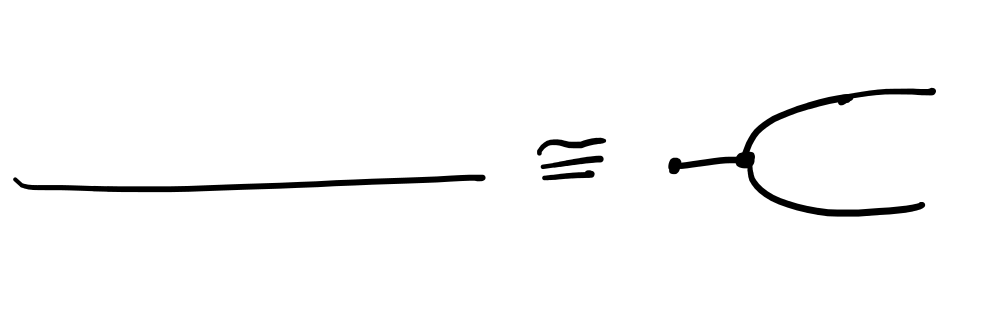
\includegraphics[width=1\linewidth]{images/States.png}
    \end{figure}
    Morphisms from the monoidal unit are called \emph{states}. This
    means that any diagram can be reorganised so that all dangling wires
    appear on one side. Collecting all dangling wires to the left and all
    generators that are morphisms from the unit object to the right, we
    obtain a diagram of the form:
    \begin{figure}[H]
        \centering
        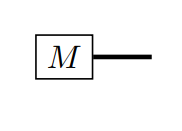
\includegraphics[width=.3\linewidth]{images//GQA/CollectDiagrams.png}
    \end{figure}
    where $M$ is a diagram of arity $0$. We now separate the $-\circ$
    generators from the remaining ones, and collect the dangling wires
    accordingly. Without loss of generality, assume there are $K$ such
    generators:
    \begin{figure}[H]
        \centering
        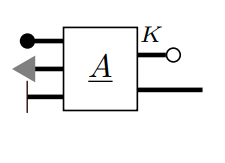
\includegraphics[width=.3\linewidth]{images//GQA/ProofNormalForm1.png}
    \end{figure}
    Here $A$ is a fragment of $\overrightarrow{\mathbf{GLA}}$ and
    therefore represents a matrix \cite{bonchi2017interacting}. To realize this, just recall that we can take the co-sum and co-copy and transform them into the copy and the sum by bending the wires with a spider.

    Applying the axioms, we derive:
    \begin{figure}[H]
        \centering
        
\includegraphics[width=1\linewidth]{images//GQA/ProofNormalForm2.png}
    \end{figure}
    We use the fact that a matrix can be decomposed into rows. We
    pick $A_1$ as the row satisfying $A_1 x = 0$ and decompose it
    into scalar components $\alpha, \beta, \gamma$ — one-dimensional
    row vectors — such that $\alpha x_1 + \beta x_2 + \gamma x_3 = 0$.
    If $\beta = 0$, the corresponding black dot generator is eliminated
    immediately:
    \begin{figure}[H]
        \centering
        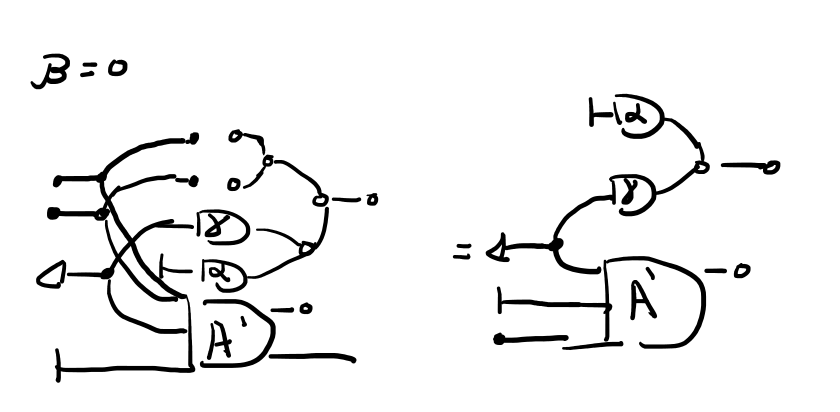
\includegraphics[width=1\linewidth]{images//GQA/ProofNormalForm3.png}
    \end{figure}
    If $\beta \neq 0$, then there exists an index $i$ such that
    $\beta_i \neq 0$, and we can eliminate one occurrence of the white
    dot and one of the black dot simultaneously:
    \begin{figure}[H]
        \centering
        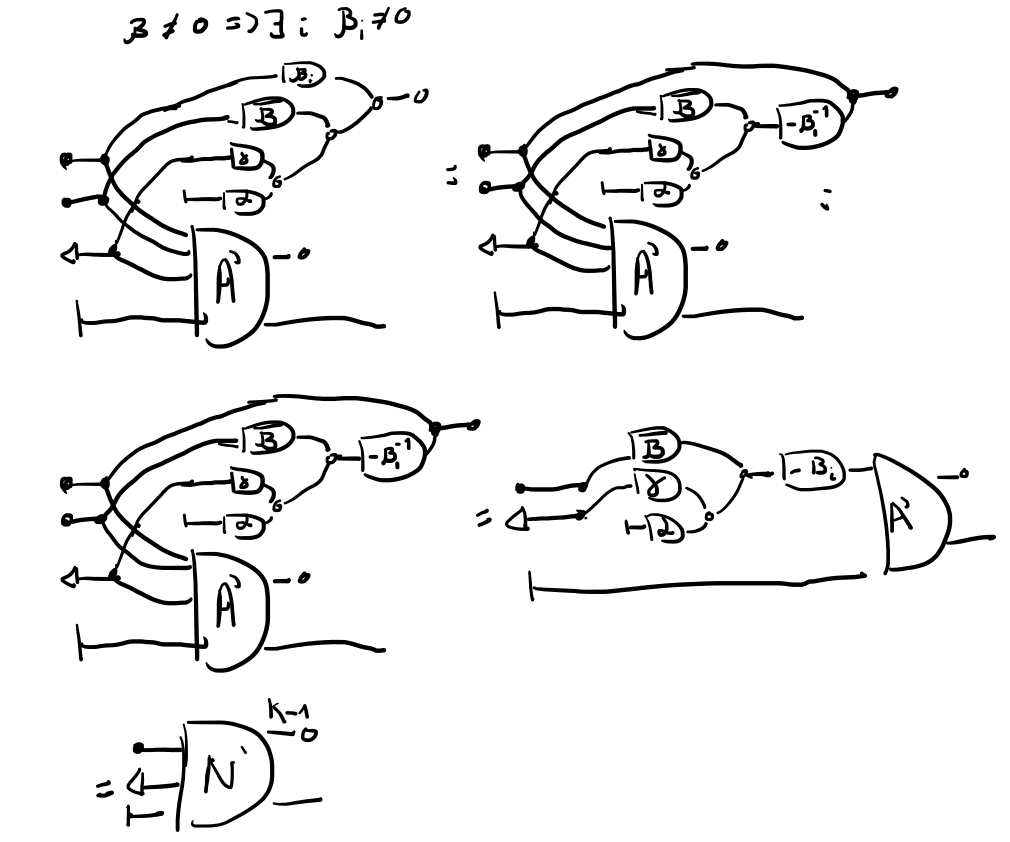
\includegraphics[width=1\linewidth]{images//GQA/ProofNormalForm4.png}
    \end{figure}
    By induction on the number of rows, we repeat this process for all
    rows with $\beta \neq 0$, leaving only rows with $\beta = 0$. The
    diagram reduces to:
    \begin{figure}[H]
        \centering
        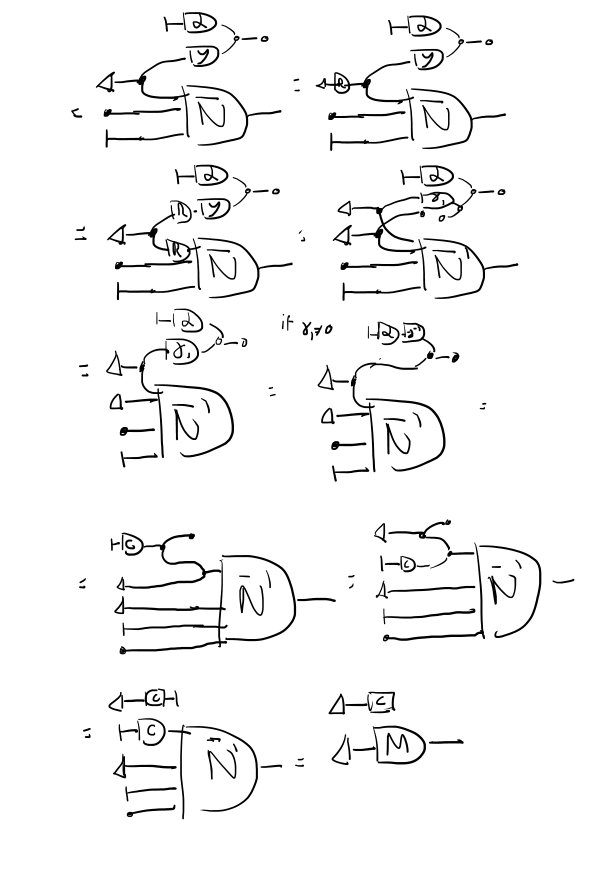
\includegraphics[width=1\linewidth]{images//GQA/ProofNormalForm5.png}
    \end{figure}
    Here $R$ is an orthogonal matrix such that
    $R\gamma = (\gamma_1, 0, \ldots, 0)$. If $\gamma_1 \neq 0$, the
    normal form is achieved. If $\gamma_1 = 0$, the wire disconnects
    trivially and we are left with:
    \begin{figure}[H]
        \centering
        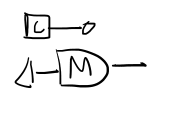
\includegraphics[width=.5\linewidth]{images//GQA/ProofNormalForm6.png}
    \end{figure}
    In both cases the diagram has been reduced to the claimed normal form
    $M' \otimes c$, completing the proof.
\end{proof}

With the normal form established, we now have all the ingredients needed
to prove the three properties — soundness, expressivity, and completeness
— that together guarantee that $\mathbf{GQA}$ is a faithful and complete
axiomatisation of $\mathbf{QuadRel}$. We treat each in turn.

\begin{lemma}[Soundness]
   If $s = t$ in $\mathrm{FreeP}_{\mathbf{GQA}}$, then $[s] = [t]$
   in $\mathbf{QuadRel}$.
\end{lemma}

\begin{proof}
    Since $\mathbf{AffRel}$ embeds into $\mathbf{QuadRel}$ via the
    indicator function, all axioms inherited from $\mathbf{GAA}$ are
    already sound in $\mathbf{QuadRel}$. It therefore suffices to verify
    soundness for the newly introduced axioms involving the gray arrow
    generator, which is done by direct computation of the corresponding
    semantic interpretations:
    \begin{figure}[H]
        \centering
        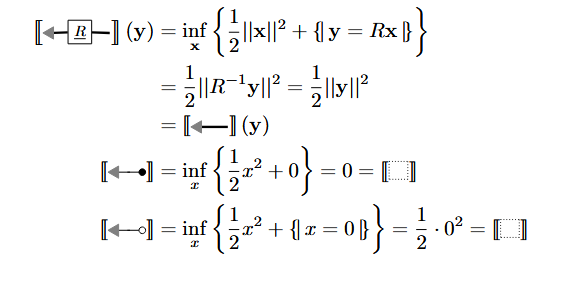
\includegraphics[width=1\linewidth]{images//GQA/SoundnessGQA.png}
    \end{figure}
\end{proof}

\begin{lemma}[Expressivity]
    For every $f : m \to n$ in $\mathbf{QuadRel}$, there exists a
    $\Sigma$-term $s : m \to n$, equivalently a morphism
    $s \in \mathrm{Hom}_{\mathrm{FreeP}_{\mathbf{GQA}}}(m,n)$,
    such that $[s] = f$.
\end{lemma}

\begin{proof}
    By Proposition~\ref{prop:PQFEquivalence}, for every non-negative
    partial quadratic function $f$ there exists an invertible coordinate
    change $g$ such that
    \[
    g(f(x_1, x_2, x_3))
    = \tfrac{1}{2}\|x_1\|^2 + \mathbf{1}_{\{0\}}(x_3),
    \]
    which is represented diagrammatically as:
    \begin{figure}[H]
        \centering
        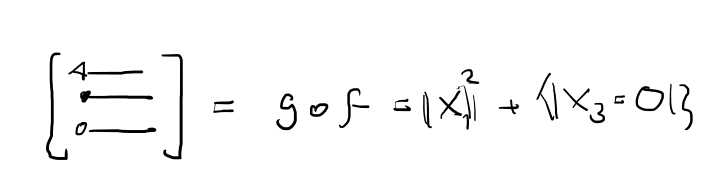
\includegraphics[width=1\linewidth]{images/GQA/PQFDiagram.png}
    \end{figure}
    Since the coordinate change $g$ is itself expressible as a morphism
    in $\mathbf{GQA}$, the general case follows by composition:
    \begin{figure}[H]
        \centering
        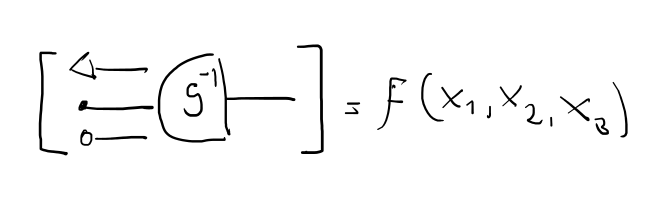
\includegraphics[width=1\linewidth]{images//GQA/ProofExpressivity.png}
    \end{figure}
\end{proof}

\begin{lemma}[Completeness]
   If $[s] = [t]$ in $\mathbf{QuadRel}$, then $s = t$ in
   $\mathrm{FreeP}_{\mathbf{GQA}}$.
\end{lemma}

\begin{proof}
    We reduce both $s$ and $t$ to their respective normal forms
    $s = M_1 \otimes c_1$ and $t = M_2 \otimes c_2$ using the Normal
    Form Theorem. Since $M_1, M_2$ lie in the fragment
    $\overrightarrow{\mathbf{GQA}} \cup \{\bullet{-}\}$,
    Lemma~\ref{rmk:normalformgqa} allows us to write them in the
    canonical block form:
    \begin{figure}[H]
        \centering
        
\includegraphics[width=0.25\linewidth]{images//GQA/ProofCompleteness1.png}
    \end{figure}
    where $D_i$ is a vector subspace, $\mu_i \in D_i^\perp$, $L_i$ is
    lower triangular, and $\operatorname{im}(L_i L_i^\top) \subseteq
    D_i^\perp$. By Proposition~\ref{prop:quadrel_equiv}, $[N_1] = [N_2]$
    if and only if $D_1 = D_2$, $\mu_1 = \mu_2$, and
    $L_1 L_1^\top = L_2 L_2^\top$.

    If $AA^\top = BB^\top$, then there exists an orthogonal matrix $R$
    such that $A = BR$, and the axioms of $\mathbf{GQA}$ allow us to
    rewrite one diagram into the other by applying the corresponding
    orthogonal transformation diagrammatically. Appealing to the
    completeness of $\mathbf{GAA}$ for the affine fragment, we conclude
    $N_1 = N_2$ in $\mathrm{FreeP}_{\mathbf{GQA}}$. Since
    $M_i = N_i \otimes c_i$ and $c_1 = c_2$ follows from
    $[s] = [t]$, we obtain $M_1 = M_2$, as desired.
\end{proof}

Combining the three lemmas, the main presentation theorem follows
immediately.

\begin{theorem}
    $\mathbf{QuadRel}$ is presented by $\mathrm{FreeP}_{\mathbf{GQA}}$.
\end{theorem}

\begin{proof}
    Soundness, expressivity, and completeness were established by the
    preceding three lemmas. Together they imply that the canonical PROP
    morphism $\mathrm{FreeP}_{\mathbf{GQA}} \to \mathbf{QuadRel}$ is
    full, faithful, and essentially surjective, hence an isomorphism of
    PROPs.
\end{proof}

\subsection{Results in GQA}

Having established that $\mathbf{GQA}$ completely axiomatises
$\mathbf{QuadRel}$, we now demonstrate the expressive power of the
calculus by deriving several non-trivial results purely through string
diagram manipulation. These propositions illustrate that the diagrammatic
language is not merely a notational device, but a genuine proof calculus
in which geometric and algebraic arguments about quadratic optimization
can be carried out compositionally. We begin with two fundamental
structural results — the expansion and contraction relations — before
moving to orthogonal projections and the generalized singular value
decomposition.

\begin{proposition}[Expansion Relation]
\leavevmode\par
\noindent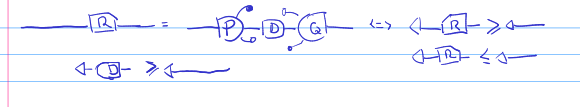
\includegraphics[width=\linewidth]{images/GQA/ExpansionRelation.png}
\end{proposition}

\begin{proof}
\leavevmode\par
\noindent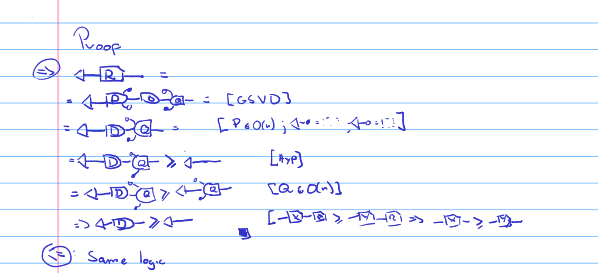
\includegraphics[width=\linewidth]{images/GQA/ProofExpansion.png}
\end{proof}

\begin{proposition}[Contraction Relation]
\leavevmode\par
\noindent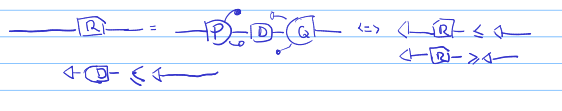
\includegraphics[width=\linewidth]{images/GQA/ContractionRelation.png}
\end{proposition}

\begin{proof}
    The proof follows by an entirely analogous diagrammatic argument to
    that of the Expansion Relation above, applying the axioms of
    $\mathbf{GQA}$ in the reverse direction.
\end{proof}

The following proposition establishes the diagrammatic representation of
orthogonal projections. This is a key result, as projections appear
naturally in least-squares problems whenever the system $Ax = b$ is
inconsistent, and the pseudoinverse computation relies essentially on
projecting onto the image of $A$.

\begin{proposition}[Matrix Projection]
    If $P$ is an orthogonal projection, then:
\leavevmode\par
\noindent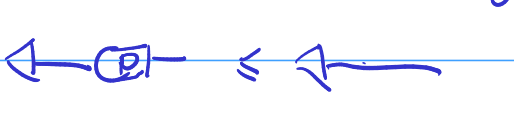
\includegraphics[width=\linewidth]{images/GQA/OrthogonalProj.png}
\end{proposition}

\begin{proof}
\leavevmode\par
\noindent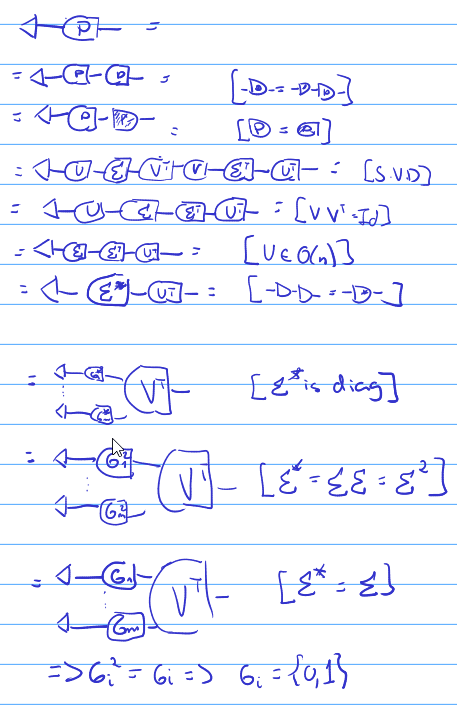
\includegraphics[width=\linewidth]{images/GQA/ProofMatrixProj.png}
\noindent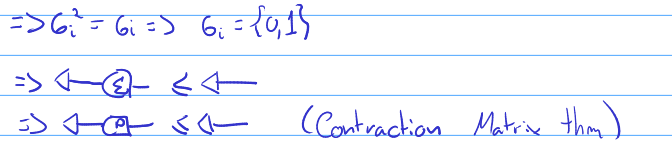
\includegraphics[width=\linewidth]{images/GQA/ProofMatrixProj2.png}
\end{proof}

The next result extends the orthogonality argument to the setting of
generalized singular value decompositions.

\begin{proposition}[GSVD Orthogonality]
\leavevmode\par
\noindent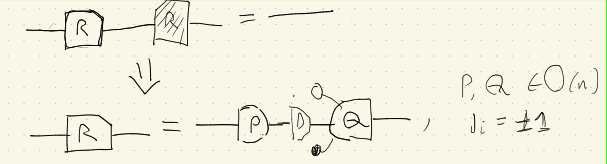
\includegraphics[width=\linewidth]{images/GQA/GSVDOrth.png}
\end{proposition}

\begin{proof}
\leavevmode\par
\noindent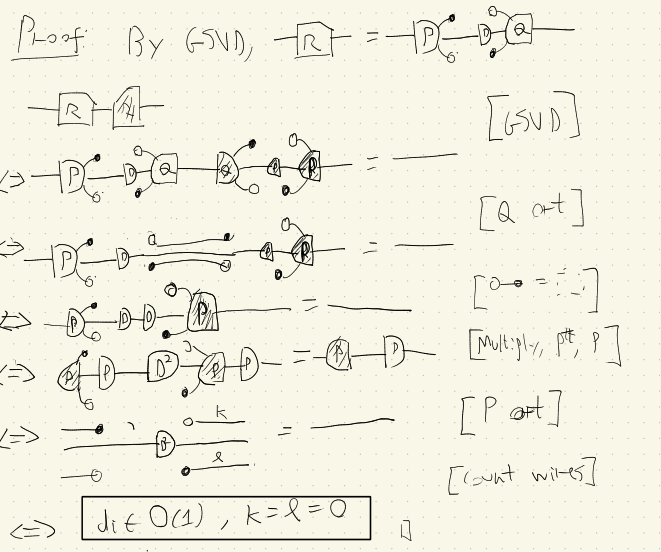
\includegraphics[width=\linewidth]{images/GQA/ProofGSVDOrth.png}
\end{proof}

Finally, the Relation Projection proposition combines the preceding
results to characterise how orthogonal projections interact with
quadratic relations.

\begin{proposition}[Relation Projection]
\leavevmode\par
\noindent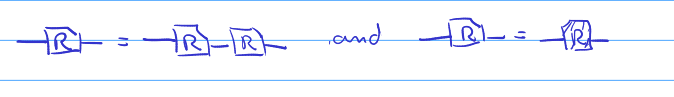
\includegraphics[width=\linewidth]{images/GQA/OrthogonalProjectionRelation.png}
\noindent
\includegraphics[width=\linewidth]{images/GQA/OrthogonalProjRel2.png}
\end{proposition}

\begin{proof}
\leavevmode\par
\noindent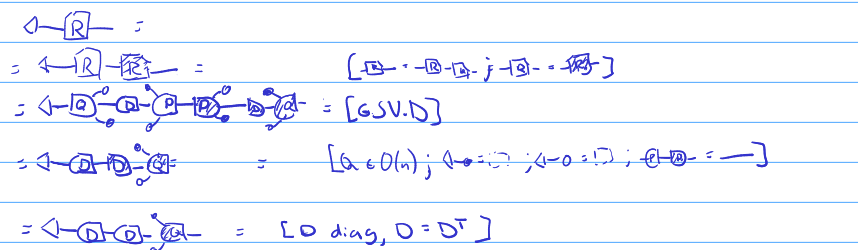
\includegraphics[width=\linewidth]{images/GQA/ProofOrthRel.png}
\noindent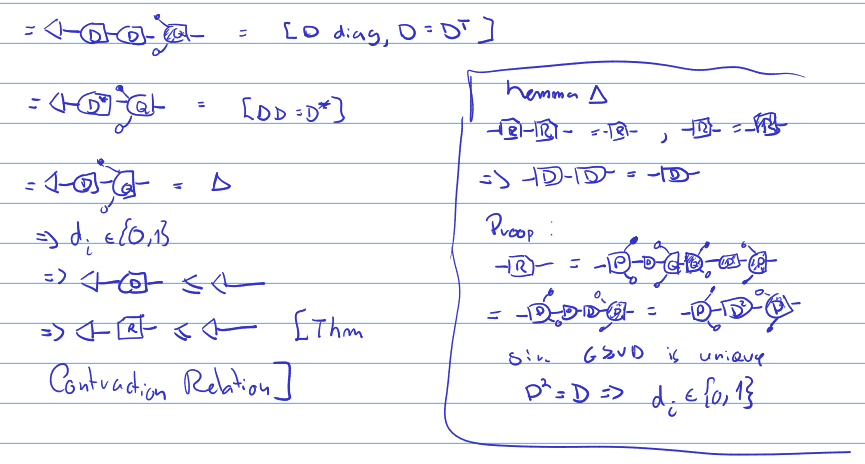
\includegraphics[width=\linewidth]{images/GQA/ProofOrthRel2.png}
\end{proof}
\begin{proposition}[The OLS estimator]

\end{proposition}
